% !TEX root = main.tex

% TODO:
% REMARK:

\section{Physical Objects Reconstruction and Selection}
\label{sec:PhysObj}

	\subsection{Vertex}
	\label{ssec:PhysObj_vertex}

		% https://iopscience.iop.org/article/10.1088/1742-6596/110/9/092009/pdf

	\subsection{Pileup Issue}
	\label{ssec:PhysObj_pu}{}

		% https://cms.cern/news/reconstructing-multitude-particle-tracks-within-cms
		Because of the high luminosity of pp collision in CMS, there are more than one pp collision occuring in every time when the the bunches cross one another. The multiple collision in one crossing event is called $\textbf{pile-up(pileup)}$. In the present, the LHC is operating at an instantaneous luminosity of $0.7\times10^{34} cm^{-2}s^{-1}$, and the proton bunches cross inside CMS every 50 ns, so there are more proton in one bunch and showing high pileup. Also, the high granularity and efficiency of CMS Tracker make them distinguish the many tracks in an event. The pileup image is shown below(Fig.\ref{PhysObj:fig:pileup_img}).

		% https://cms.cern/news/reconstructing-multitude-particle-tracks-within-cms
		\begin{figure}[H]
		\centering{}
	    	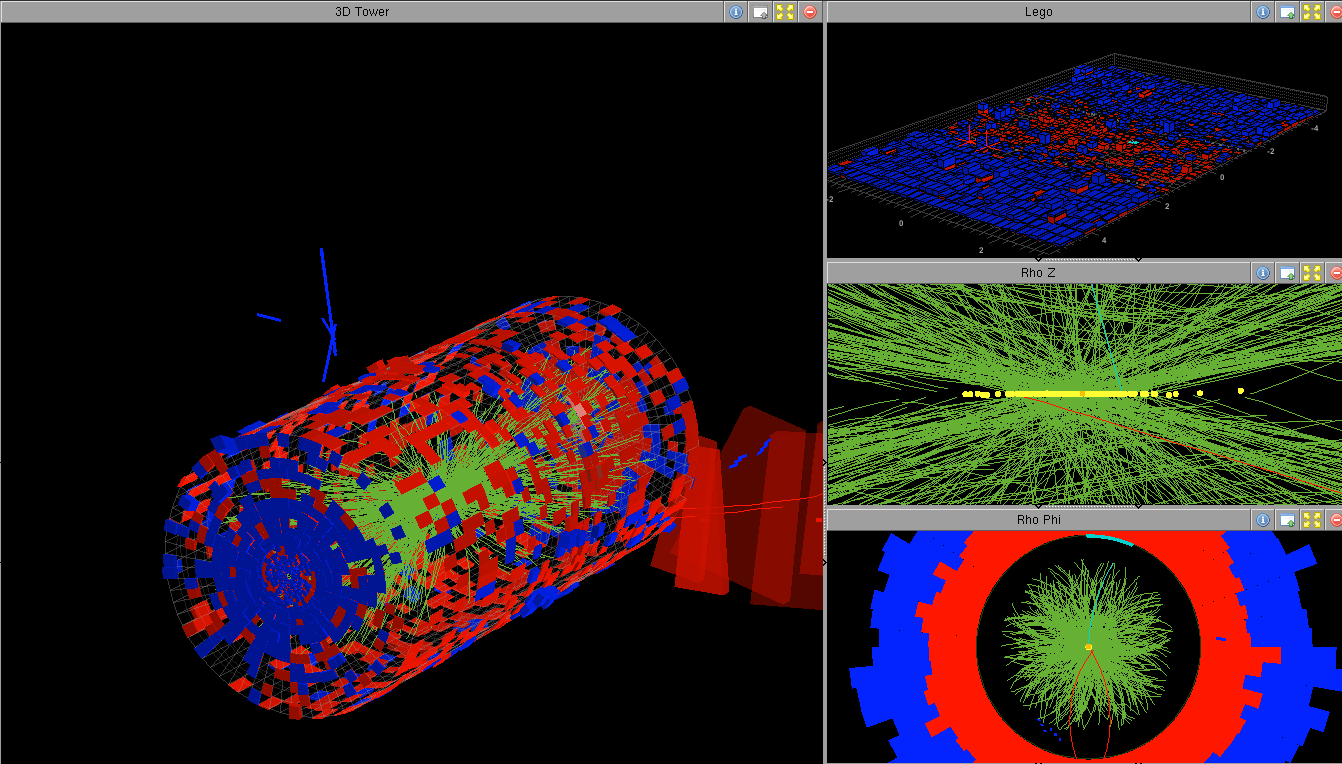
\includegraphics[width=0.85\textwidth]{Figures/PhysObj/pileup_image.png}\\
		\caption{78 reconstructed vertices in one crossing from high pileup run (3D, lego, on Pho-z plane, on Rho-Phi plane)}
		\label{PhysObj:fig:pileup_img}
		\end{figure}
		\FloatBarrier



	\subsection{Lepton}
	\label{ssec:PhysObj_lep}

		The selected lepton in the analysis is required to obey the criteria of one passed $\emph{selected lepton}$ and zero $\emph{veto lepton}$ passed. The veto criteria means that there would be no lepton passing the veto criteria except the selected one. In other words, the veto criteria can filter the physical objects which are lepton-like but not really like after reconstructed from particle level to detector level. The selected criteria corresponds to tight lepton's criteria, and veto criteria follows loose lepton's criteria:

		\subsubsection{Muon}
		\label{sssec:Muon}
			

		\subsubsection{Electron}
		\label{sssec:Electron}

	\subsection{Jet}
	\label{ssec:PhysObj_jet}

		\subsubsection{B-tagged jet}
		\label{sssec:bjet}


	\subsection{Trigger}
	\label{ssec:PhysObj_trg}





\FloatBarrier
